\section{Análises}
\subsection{Análise da Arquitetura}

\begin{table}[h!]
  \centering
  \begin{tabular}{lll}
    \toprule
    \textbf{Nome}                  & \textbf{Back-end} & \textbf{Android} \\
    \midrule
    Linguagem de Programação       & Ruby              & Java             \\
    Framework                      & Ruby on Rails     & Android SDK      \\
    Arquitetura de Software        & MVC               & --               \\
    Comunicação (API)\footnotemark & RESTful (JSON)    & RESTful(JSON)    \\
    Servidor HTTP                  & Apache            & -                \\
    Banco de dados                 & PostgreSQL        & SQLite           \\
    \bottomrule
  \end{tabular}

  \caption{Especificações do back-end e do aplicativo Android.}
  \label{tab:back-end-espec}
\end{table}

\footnotetext{Comunicação entre o \emph{back-end} e o \emph{front-end}.}

O iNaturalist é um sistema complexo e com muitos recursos, que estendem desde o armazenamento dos dados, através das observações, até suas ferramentas de análises, pela sua interface web. A tabela \ref{tab:back-end-espec} mostra as principais características, como as linguagens e arquiteturas utilizadas.

Tecnologias modernas e de código aberto foram muito bem exploradas no desenvolvimeto do sistema, como visto na tabela \ref{tab:back-end-espec}. \emph{Ruby on Rails} é uma \emph{framework} de código aberto, robusta e estável. É usada por grandes nomes como GitHub, Shopify, SoundCloud, Airbnb e outras.

\begin{figure}[h!]
  \centering
  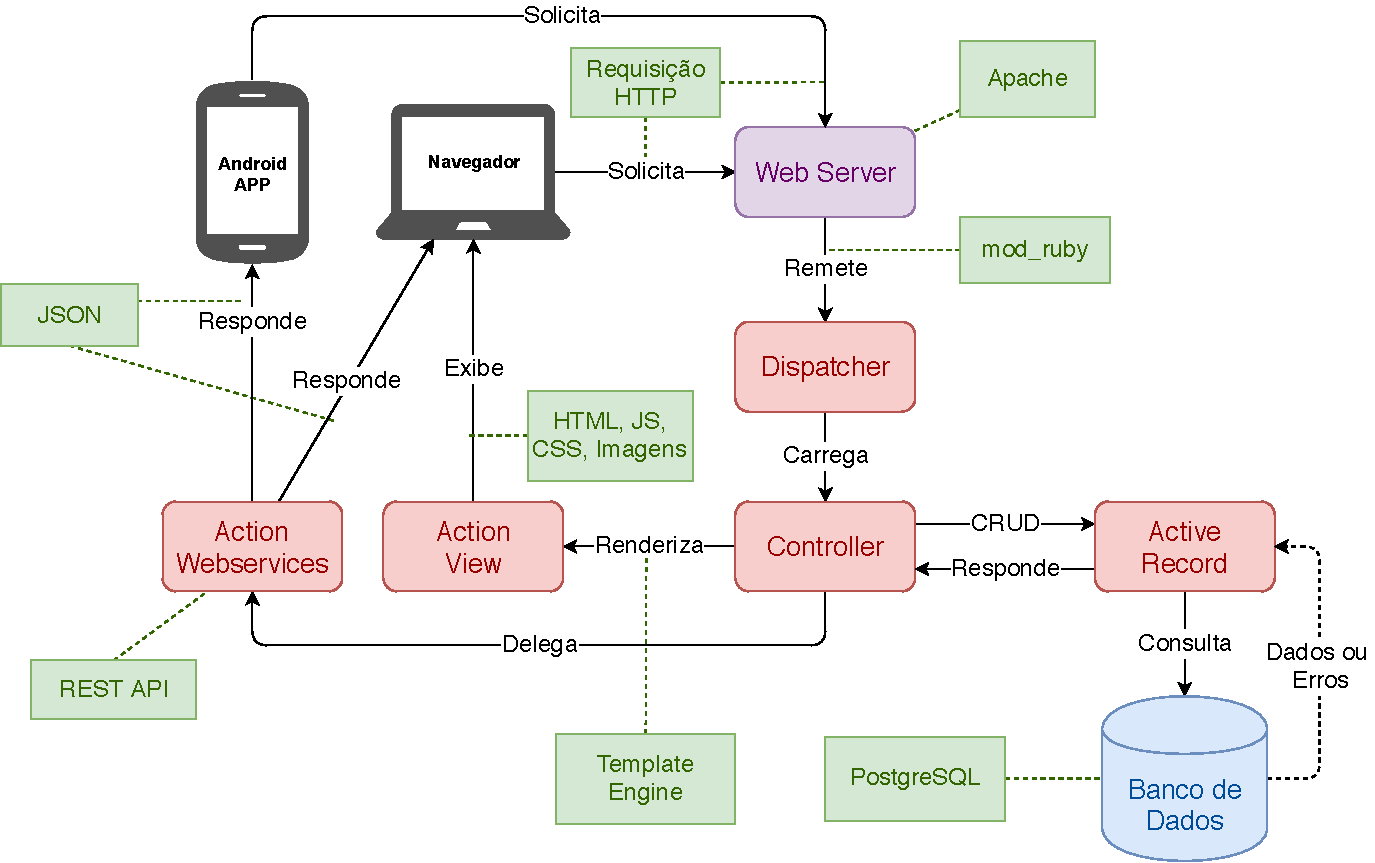
\includegraphics[width=\textwidth]{figures/arch_diagram.pdf}
  \caption{Diagrama simplificado da arquitetura do iNaturalist.}
  \label{fig:arch}
\end{figure}

É notável, também, o uso arquitetura de software MVC (Model-View-Controler), que é a arquitetura padrão do \emph{Ruby on Rails}. Ela divide a aplicação em três camadas de abstração interconectadas: modelo, visão e controlador. Ela é usada para separar representações internas de informações da representação final para o usuário do sistema. Isso organiza a criação de interfaces gráficas, uma vez que a camada de visualização está separada da lógica interna do sistema.

A figura \ref{fig:arch} mostra um diagrama simplificado da arquitetura do iNaturalist, nele é representado os componentes do sistema e as camadas de abstração da framework, mostrando  como o \emph{back-end} interage com o usuário dependendo do dispositivo usado para acessar os serviços.

Os blocos vermelhos são camadas de abstração do \emph{Ruby on Rails}, que são representadas por classes. Os blocos verdes são informações adicionais de algum componente ou processo. E os demais blocos são componentes do sistema. Alguns dos elementos do diagrama serão descritos a seguir.

\begin{description}
  \item[Web Server] \hfill \\ Componente do sistema responsável por monitorar as requisições HTTP feitas ao servidor e encaminhar para a aplicação Ruby. Sua importância está no gerenciamento dos recursos do sistema, criando vários processos da aplicação para que seja possível executar requisições em paralelo.
  \item[Dispatcher] \hfill \\ É uma das primeiras classes do fluxo de uma requisição. Ela que faz interface entre a rede e o sistema, recebendo a requisição HTTP do \emph{Web Server} e instanciando o controlador da respectiva rota\footnote{Neste contexto, rota está relacionada com o caminho completo da URL. Cada caminho tem um controlador associado, que pode renderizar uma página, fazer persistência de dados e etc.}.
  \item[Controller] \hfill \\ É implementada a lógica de uma ou de um conjunto de rotas identificadas por um padrão.
  \item[Active Record] \hfill \\ Responsável por representar e manipular as tabelas do banco de dados.
  \item[Action View] \hfill \\ É a classe de visualização e, portanto, é uma das últimas classe do fluxo de uma requisição. Ela recebe os dados do controlador manipula o template para renderizar uma página.
  \item[Action Webservices] \hfill \\ É uma classe de apoio do \emph{Ruby on Rails} para facilitar a criação de \emph{Web Services} interoperáveis com a \emph{framework}. Assim como a \texttt{Action View}, ela também está no final do fluxo de uma requisição, mas ao invés de renderizar uma página, ela processa e reponde requisições feitas pela API.
\end{description}

A arquitetura deste sistema é monolítica. Uma das principais características é que o sistema é segmentado por partes responsáveis por uma tarefa específica e estas partes são interconectadas. É possível observar isso analisando figura \ref{fig:arch} e a descrição dos elementos.

Alguns pontos positivos da arquiterura monolítica são:

\begin{enumerate}
  \item Desenvolvimento: no princípio, o desenvolvimento é muito simples, pois todo \emph{codebase} está em uma mesma linguagem e em um mesmo ambiente.
  \item Implantação: como todo código está em um mesmo ambiente, a implantação é simples: basta fazer uma cópia para o servidor.
  \item Escalamento horizontal: para escalar o sistema, basta rodar múltiplas cópias atrás de um balanceador de carga.
\end{enumerate}

Já alguns dos pontos negativos são:

\begin{enumerate}
  \item Manuntenção: se a aplicação fica muito grande e complexa, fazer mudanças rapidatemente e corretamente torna-se um desafio, pois o encapsulamento de código é usado extensivamente pela arquitetura para separar o código em níveis de abstração, o que torna difícil fazer uma modificação sem gerar efeitos colaterais em outras partes do sistema.
  \item Confiabilidade: um \emph{bug} em qualquer módulo (ex: vazamento de memória) pode potencialmente derrubar todo processo. E, como todas as instâncias da aplicação são idênticas, este \emph{bug} pode afetar o desenpenho de todo sistema.
  \item Modernização: pode ser difícil novas tecnologias em aplicações monolíticas, já que modificações na linguagem ou na \emph{framework} afeta toda a aplicação.
\end{enumerate}

Com esses apontamentos, é certo concluir que a arquitetura adotada pelo projeto facilita a implantação da aplicação no servidor. Mas, por outro lado, existe um custo para fazer uma modificação no código, principalmente se a modificação envolver vários níveis de abstração.

Modificações como tradução ou qualquer outra na camada de visualização pode ser facilmente implementada, mas ao chegar em camadas mais baixas, como a lógica de negócio ou modelagem dos dados, é difícil fazer modificações sem romper a compatibilidade com o sistema original, que, por sua vez, também é modificado periodicamente.

\subsection{Análise dos Novos Recursos}

A possibilidade de fazer observações em um local mesmo que o smartphone não esteja conectado à internet é um ponto forte do aplicativo e garante que as observações posam ser feitas de qualquer lugar. Os dados ficam armazenados na memória interna do aparelho e, quando conectado à rede, os dados são enviados para o servidor.

A partir das informações geográficas de latitude e longitude obtidas pelo próprio sensor do smartphone ou fornecidas pelo voluntário, assim que uma observação é enviada para o servidor, é adicionado um ponto no mapa representando a localização do espécime observado. Clicando sobre o ponto é possível obter informações detalhadas da observação. Além disso, para aprimorar a análise dos dados, é possível aplicar combinações de filtros que restringem a apresentação das observações no mapa. Essas restrições podem ser de acordo com o táxon, data ou local da observação. Assim, é possível observar a ocorrência de uma espécie em uma determinada época do ano ou sua presença em uma determinada região. Diversas combinações podem ser feitas de acordo com a necessidade da análise.

A estrutura de rede social cria vínculos entre os voluntários e pesquisadores e propicia o engajamento de mais voluntários à observação da natureza. Além disso, profissionais podem revisar a classificação do espécime feita pelos voluntários e sinalizar algo que esteja identificado incorretamente.

% • Uso de internet no 'auto-complete' e possível implementação offline.

% • Auto-complete otimizado para pesquisas utilizando nome popular em português

% • Ventagens da implementação dos 'badges' ('Crowdsourcing the identification of organisms: A case-study of iSpot.').
